\subsection{Properties of Functions: Extremas}
\begin{definition}[Local/Relative Maximum]
  The highest point in a specific region or a small interval of a function.
  $$f(x) \le f(c) \, ... \, c \, is \, a \, local \, max$$
  Where functions changes from increasing to decreasing.
\end{definition}

\begin{definition}[Local/Relative Minimum]
  The lowest point in a specifis region or a small interval of a function.
  $$f(x) \ge f(c) \, ... \, c \, is \, a \, local \, min$$
  Where functions changes from decreasing to increasing.
\end{definition}

\textbf{Note: } Endpoints are not allowed for Local minimum or maximum. But it is allowed for absolute minimum or maximum.

\begin{definition}[Absolute Maximum]
  Highest output on graph.
\end{definition}

\begin{definition}[Absolute Minimum]
  Lowest output on graph
\end{definition}

\textbf{Note: } Every continous closed interval ``[,]`` will guarantee we have an absolute max and an absolute min.

\begin{example}[Graph]
  \hfill
  \begin{center}
    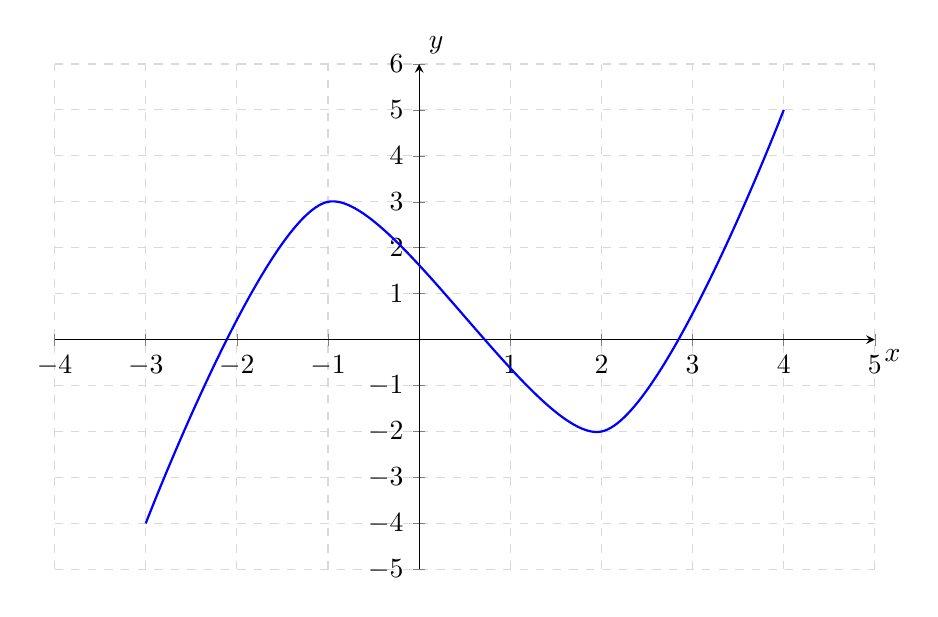
\begin{tikzpicture}
      \begin{axis} [
	  width = 12cm,
	  height = 8cm,
	  axis lines = center,
	  xlabel = $x$,
	  ylabel = $y$,
	  xmin = -4, xmax = 5,
	  ymin = -5, ymax = 6,
	  grid = both,
	  grid style = {dashed, gray!30},
	  xtick = {-4,-3,...,5},
	  ytick = {-5,-4,...,6},
	  xlabel style = {at={(ticklabel* cs:1)}, anchor=north west},
	  ylabel style = {at={(ticklabel* cs:1)}, anchor=south west}
	]
	\addplot [smooth, thick, blue] coordinates {
	  (-3, -4) 
	  (-1, 3) 
	  (2, -2) 
	  (4, 5)
	};
      \end{axis}
    \end{tikzpicture}
  \end{center}
  \begin{enumerate}
  \item Local Minimum: $-2 \, @ \, (2, -2)$
  \item Local Maximum: $3 \, @ \, (-1, 3)$
  \item Absolute Minimum: $-4 \, @ \, (-3, -4)$
  \item Absolute Maximum: $5 \, @ \, (4, 5)$
  \end{enumerate}
\end{example}
